
%(BEGIN_QUESTION)
% Copyright 2006, Tony R. Kuphaldt, released under the Creative Commons Attribution License (v 1.0)
% This means you may do almost anything with this work of mine, so long as you give me proper credit

Et alternativ til å bruke trykkavlastningsventil for trykkstyring i et hydraulikksystem er å bruke en {\it variabel-fortrengningspumpe} med hydraulisk tilbakekobling:

$$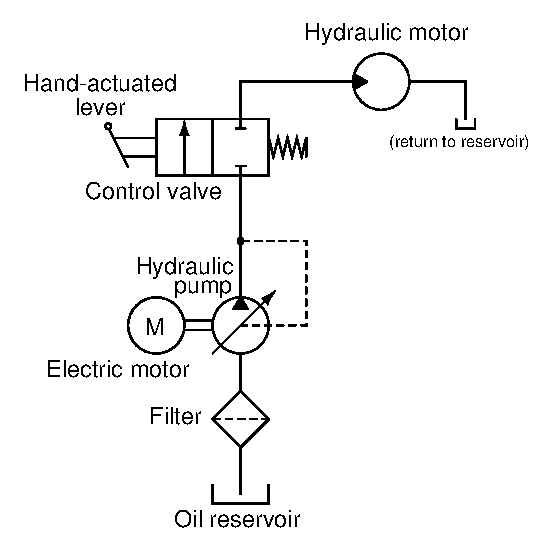
\includegraphics[width=15.5cm]{i00763x01.eps}$$

Når hydraulikktrykket øker, justerer pumpemekanismen automatisk til lavere volumfortrengning per omdreining. Forklar hvordan dette regulerer trykket, og hvorfor det sparer energi sammenlignet med mer tradisjonelt oppsett med konstant-fortrengningspumpe kombinert med trykkavlastningsventil.

\underbar{file i00763}
%(END_QUESTION)





%(BEGIN_ANSWER)

I stedet for å sløse bort ubrukt hydraulisk energi i en trykkavlastningsventil, reduserer dette systemet mengden hydraulisk energi som tilføres når den ikke trengs.

\vskip 10pt

Oppfølgingsspørsmål: En vanlig utforming av variabel-fortrengnings hydraulikkpumpe (og motor!) er {\it swash plate}-typen, der vinkelen på swash-platen endres for å endre fortrengningen per omdreining. Undersøk denne pumpetypen og forklar hvordan den fungerer.

%(END_ANSWER)





%(BEGIN_NOTES)

%INDEX% Mekanikk, fluidkraftsystemer: variabel fortrengningspumpe for trykkregulering

%(END_NOTES)


